\subsection{\name{} Runtime}\label{sec:runtime}

\begin{figure}[t!]
	\centering
	\scalebox{1}{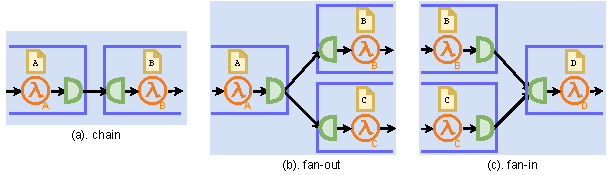
\includegraphics[width=\columnwidth]{figures/deorc-patterns.pdf}}
	\caption{\deorc{} implements transitions in a decentralized manner where
the egress on the source function(s) and ingress on the target function(s)
work together to execute the orchestration. \shadi{does this figure add value given you have Fig 1. you can probably combine the patterns there ans name them there and reuse that figure.}}
	\label{fig:transition}
\end{figure}

\begin{figure}[]
    \begin{minted}[
    frame=single,
    fontsize=\scriptsize
  ]{json}
{
    "Data": {
        "Source": "http | dynamodb | s3 | ...",
        "Value": "<object> | [<pointers>]"
    },
    "Session": "uuid",
    "Fan-out": {
        "Index": "int",
        "Size": "int",
        "OuterLoop": {
            "Index": "int",
            "Size": "int"
        }
    }
}
    \end{minted}
    \caption{\name{} runtime input payload schema}
    \label{fig:input-format}
\end{figure}

The second challenge of \name{} is to efficiently implement decentralized
orchestration. \name{} designs a decentralized orchestrator (\deorc) that
consists of an ingress and an egress component and can run in-situ with
constituent user functions. \deorc{} transparently interposes on user code
entry and exit so that it does not change how developers write application
code.

The primary purpose of \deorc{} is to interpret IR configurations and implement
transitions with platform-specific APIs. In particular, \deorc{} implements
transitions in a decentralized manner where the egress on the source
function(s) and ingress on the target function(s) work together to execute the
transition.

A key requirement of \deorc's design is to only use the basic serverless
abstraction without relying on any specialized APIs. Therefore, we designed
\deorc{} such that it only depends on two serverless components that are
universally supported by all platforms: i. a FaaS system that supports
asynchronous invocation of functions (e.g., AWS Lambda, Azure Functions,
Google Cloud Funtions, Openwhisk) and ii. a strongly consistent data store
that supports conditional write operations (e.g., DynamoDB, Cosmos DB).

Figure~\ref{fig:transition} depicts how \deorc{} executes \texttt{chain},
\texttt{map} and \texttt{fan-in}. The other patterns described in
\S\ref{sec:ir} are variations of these three patterns.

\paragraph{chain} 

The \texttt{chain} pattern involves one egress on source function and one
ingress on the target function. When the \texttt{Next} field of the source
function's \name{} config contains a single object whose \texttt{InputType} is
\texttt{Scalar}, the \deorc{} egress simply invokes the target function with
the source function's user code's output. \deorc{} uses asynchronous
invocation to avoid waiting and idle-billing and a particular input payload
schema in JSON (Figure~\ref{fig:input-format}) that contains \name{} runtime
metadata.

When the target function is invoked, the input is first received by the \deorc{}
ingress. The ingress uses the \texttt{Data} field to read the user function's
input data. If the \texttt{Source} is \texttt{http}, the input data is
directly embedded in the \texttt{Value} field. Otherwise,
\name{} uses the pointers in \texttt{Value} to read the input data from the
intermediary data store. Finally, ingress calls its user function and passes
it the input.

\paragraph{fan-out}

The \texttt{fan-out} pattern involves one egress on the source function and
many ingresses on the target functions.

Similar to chaining, the egress asynchronously invoke each target and the
ingresses on targets read the input data sent from the source and passes it to
its user function.

\texttt{map} is a simple variation of \texttt{fan-out} where the egress treats
its user code output as an iterable. \texttt{branch} is another variation
where the egress first evaluates the boolean condition in \texttt{Conditional}
before invoke the target function in that branch.

\paragraph{fan-in}

The \texttt{fan-in} pattern involves one ingress node and many egress nodes.
It is the main complexity of decentralized orchestration as we want to ensure
that the transition is \emph{wait-free} to avoid idle-billing. In particular,
we want to invoke the sink function only when all upstream functions have
completed so that the sink function does have to be spun up ahead of time and
wait for upstream functions to finish. Moreover, the upstream functions should
simply terminates when done instead of waiting for each other either.

To achieve this, the \deorc{} egress always writes the output of its user
function to a data store when its \name{} config has a \texttt{InputType} of
\texttt{Fan-in}. This serves two purposes: (1). it allows any of the upstream
functions to access the output of other upstream functions (2). it signals the
completion of a function. This way, each egress can simply writes its output
and terminate. Other egress nodes can still access completed egress' data
after they terminate. Any one of the egress can invoke the sink function. And
any one of the egress can see if other egress has completed or not.

Strongly consistent data store is important because it prevents the
scenarios where all egress have written outputs but none of them sees that all
have completed, which results in the sink function never invoked.

Additionally, \texttt{fan-in} makes sure that when the sink function is
invoked, it is invoked only once. \name{} achieves this by having the egress
nodes synchronize with each other via the same data store such that only the
last-to-finish egress invokes the sink function. Synchronization is done with
atomic read-after-write over a single object. Specific implementation depends
on the data store and we discuss the details in \S\ref{sec:impl}.

The last-to-finish egress invokes the sink function with a vector of pointers
to each upstream function's stored output. The pointers are the in same order
as the vector of upstream function names. The ingress on the sink function
dereferences each point by reading from the data store and passes a vector of
output values to its user function.


\subsubsection{Runtime Metadata}

To support a rich variety of orchestration patterns, \name{} requires a
specific input payload schema in JSON (Figure~\ref{fig:input-format}) that
contains \name{} runtime metadata. In particular, \name{} uses the
\texttt{Fan-out} field to store branch indexes. The \texttt{Fan-out} field
contains a recursive \texttt{OuterLoop} field that \name{} uses to support
nest fan-outs. The \texttt{\$0} and \texttt{\$size} variable in
\name{} IR (\S\ref{sec:ir}) refers to the \texttt{Index}  and \texttt{Size}
field of the top-level \texttt{Fan-out} field.

The runtime additionally uses a \texttt{Session} field to support concurrent
invocations of the same workflow. The \texttt{Session} field is a UUID string
that is unique to a workflow invocation and shared by all constituent function
instances in the invocation. Function checkpoint names
(\S\ref{sec:exec-gntee}) are prefixed by the \texttt{Session} string so that
concurrently invocations do not overwrite each other's data. We discuss
\name{} checkpoints and execution guarantees details in the next section.